\section{Справочные сведения}\label{sec:general_information}
	\subsection{Общие сведения о походе}\label{subsec:general_information}
		\begin{longtable}{|>{\centering\arraybackslash} m{6.1cm}|>{\centering\arraybackslash} m{10cm}|} \hline
			Район похода														&	Российская Федерация, Кавказ (Безенги,~Приэльбрусье)						\\ \hline
			Вид туризма															&	Горный																		\\ \hline
			Категория сложности похода											&	Третья																		\\ \hline
			Проводящая организация												&	Горный турклуб МГУ, г.~Москва												\\ \hline
			Руководитель														&	Чашникова Анастасия Алекссандровна 											\\ \hline
			Контакты руководителя												&	тел.~+7(950)~816-39-44 e-mail:~chashni98@gmail.com 							\\ \hline
			Сроки активной части похода полные \newline (от Москвы до Москвы)	&	с 30 июня по 18 июля 2024 года \textit{(с~28~июня~по~20~июля~2024~года)}	\\ \hline
			Протяженность маршрута (по карте)									&	158.1\,км (163.6\,км с учётом радиальных выходов для части группы)			\\ \hline
			Длина маршрута с учётом $k = 1.1$									&	180\,км (из них в зачёт~-- 159.4\,км)										\\ \hline
			Продолжительность активной части									&	19 дней																		\\ \hline
			Суммарный набор/сброс, м											&	+13200/-13530																\\ \hline
			Максимальная высота													&	4370\,м (гребень в.~Башхауз)														\\ \hline
			Максимальная высота ночёвки											&	4185\,м (пер.~Тютю Зап.)													\\ \hline
		\end{longtable}\fxnote{Поправить километраж}
	
	
	\subsection{Запланированная нитка маршрута}\label{subsec:planned_route}
		\renewcommand{\bfdefault}{bx}
		\textit{
			Т/б~Уштулу~"---
			\fxnote{Поправить тире! не видны на нормальном масштабе!}
			\hyperref[subsec:main_obstacles]{пер.~Штулу + п.~Штулу (1А, рад.)}~"---
			д.р.~Карасу~"---
			приют Уштулу~"---
			д.р.~Черек Балкарский~"---
			д.р.~Тютюнсу~"---
			\hyperref[subsec:main_obstacles]{пер.~Туристов Грузии + пер.~Ашинова (1Б)}~"---
			лед.~Крумкол~"---
			\hyperref[subsec:main_obstacles]{пер.~Спартак + п.~Башхауз + пер.~МВТУ (2А)}~"---
			а/л~Безенги~"---
			\hyperref[subsec:main_obstacles]{пер.~Столбовой (2А)}~"---
			\hyperref[subsec:main_obstacles]{пер.~Тютюргу (1Б)}~"---
			\hyperref[subsec:main_obstacles]{пер.~Шаурту + п. МВТУ (2А)}~"---
			лед.~Шаурту~"---
			д.р.~Тютюргу~"---
			д.р.~Гара-Аузу-Су~"---
			д.р.~Башиль-Аузу-Су~"---
			т/б Башиль~"---
			д/р~Джайлык-Су~"---
			лед.~Джайлык~"---
			\hyperref[subsec:main_obstacles]{пер.~Кенчат + п.~Кенчатбаши + пер.~Килар (2А)}~"---
			лед.~Кенчат Западный~"---
			ночевки Тютю нижние~"---
			\hyperref[subsec:main_obstacles]{пер.~Тютю Зап. + п.~Тютюбаши 2-ая Зап. + пер.~Куллумкол + пер.~Шогенцукова (2А)}~"---
			д/р~Куллумкол-Су~"---
			а/л~Джайлык~"---
			Верхний Баксан.
			}\fxnote{Поправить ссылки!}
	
	\subsection{Пройденная нитка маршрута}\label{subsec:real_route}
		\textit{
			Т/б~Уштулу~"---
			\hyperref[subsec:main_obstacles]{пер.~Штулу + п.~Штулу (1А, рад.)}~"---
			д.р.~Карасу~"---
			приют Уштулу~"---
			д.р.~Черек Балкарский~"---
			д.р.~Тютюнсу~"---
			\hyperref[subsec:main_obstacles]{пер.~Туристов Грузии + пер.~Ашинова (1Б)}~"---
			лед.~Крумкол~"---
			\hyperref[subsec:main_obstacles]{пер.~Спартак + п.~Башхауз + пер.~МВТУ (2А)}~"---
			а/л~Безенги~"---
			\hyperref[subsec:main_obstacles]{пер.~Столбовой (2А)}~"---
			\hyperref[subsec:main_obstacles]{пер.~Тютюргу (1Б)}~"---
			\hyperref[subsec:main_obstacles]{пер.~Шаурту (2А)}~"---
			лед.~Шаурту~"---
			д.р.~Тютюргу~"---
			д.р.~Гара-Аузу-Су~"---
			д.р.~Башиль-Аузу-Су~"---
			т/б Башиль~"---
			д/р~Джайлык-Су~"---
			лед.~Джайлык~"---
			\hyperref[subsec:main_obstacles]{пер.~Надежда (1Б, п/п) + пер.~Кенчат + п.~Кенчатбаши (2А, рад.)}~"---
			\hyperref[subsec:main_obstacles]{пер.~Килар (1Б)}~"---
			лед.~Кенчат Западный~"---
			ночевки Тютю нижние~"---
			\hyperref[subsec:main_obstacles]{пер.~Тютю Зап. + п.~Тютюбаши 2-ая Зап. + пер.~Куллумкол + пер.~Шогенцукова (2А)}~"---
			д/р~Куллумкол-Су~"---
			а/л~Джайлык~"---
			Верхний Баксан.
			}\fxnote{Поправить ссылки!}
		\renewcommand{\bfdefault}{b}

		Маршрут пройден с изменениями, подробнее см. \ref{subsec:changes_of_way}.

	
	\subsection{Определяющие препятствия}\label{subsec:main_obstacles}
		\begin{longtable}{|>{\centering\arraybackslash}m{5.5cm}|>{\centering\arraybackslash}m{1.0cm}|>{\centering\arraybackslash}m{1.6cm}|>{\centering\arraybackslash}m{7cm}|>{\centering\arraybackslash}m{1.7cm}|} \hline
			Препятствие																																			&	К. т.	&	Высота				&	Характер склонов	&	ЧХВ	\\ \hline
			\hyperref[subsec:main_obstacles]{Пер.~Штулу~+ п.~Штулу}														\newline\textit{радиально с запада}		&	1А		&	3570				&	травянисто-земляной склон до $20^\circ$ , короткие участки снежников до $15^\circ$ 				&		\\ \hline
			\hyperref[subsec:main_obstacles]{Пер.~Туристов Грузии~+ пер.~Ашинова}										\newline\textit{с севера на юг}			&	1Б		&	3640 3720			&						&		\\ \hline
			\hyperref[subsec:main_obstacles]{Пер.~Спартак~+ п.~Башхауз~+ пер.~МВТУ}										\newline\textit{с севера на юг}			&	2А		&	4090 4410 4215		&						&		\\ \hline
			\hyperref[subsec:main_obstacles]{Пер.~Столбовой}															\newline\textit{с востока на запад}		&	2А		&	3690				&						&		\\ \hline
			\hyperref[subsec:main_obstacles]{Пер.~Тютюргу}																\newline\textit{с севера на юг}			&	1Б		&	3835				&						&		\\ \hline
			\hyperref[subsec:main_obstacles]{Пер.~Шаурту}																\newline\textit{с севера на юг}			&	2А		&	4085				&						&		\\ \hline
			\hyperref[subsec:main_obstacles]{Пер.~Кенчат~+ п.~Кенчатбаши}												\newline\textit{радиально с востока}	&	2А		&	3905 4090			&						&		\\ \hline
			\hyperref[subsec:main_obstacles]{Пер.~Килар}																\newline\textit{с востока на запад}		&	1Б		&	3885				&						&		\\ \hline
			\hyperref[subsec:main_obstacles]{Пер.~Тютю~Зап.~+ п.~Тютюбаши 2~Зап.~+ пер.~Куллумкол~+ пер.~Шогенцукова}	\newline\textit{с севера на юг}			&	2А		&	4185 4300 3915 3590	&						&		\\ \hline
		\end{longtable}\fxnote{Доделать таблицу}
		

	\subsection{Состав группы}\label{subsec:group_composition}
		\begin{longtable}{|>{\centering\arraybackslash} m{3.5cm}|>{\centering\arraybackslash} m{3.6cm}|>{\centering\arraybackslash} m{3.5cm}|>{\centering\arraybackslash} m{2.5cm}|>{\centering\arraybackslash} m{2.5cm}|}\hline
			Фотография																																	&	ФИО										&	Должность					&	Год рождения	&	Опыт		\\ \hline
			\raisebox{-0.05\height}{\rule{0pt}{155pt}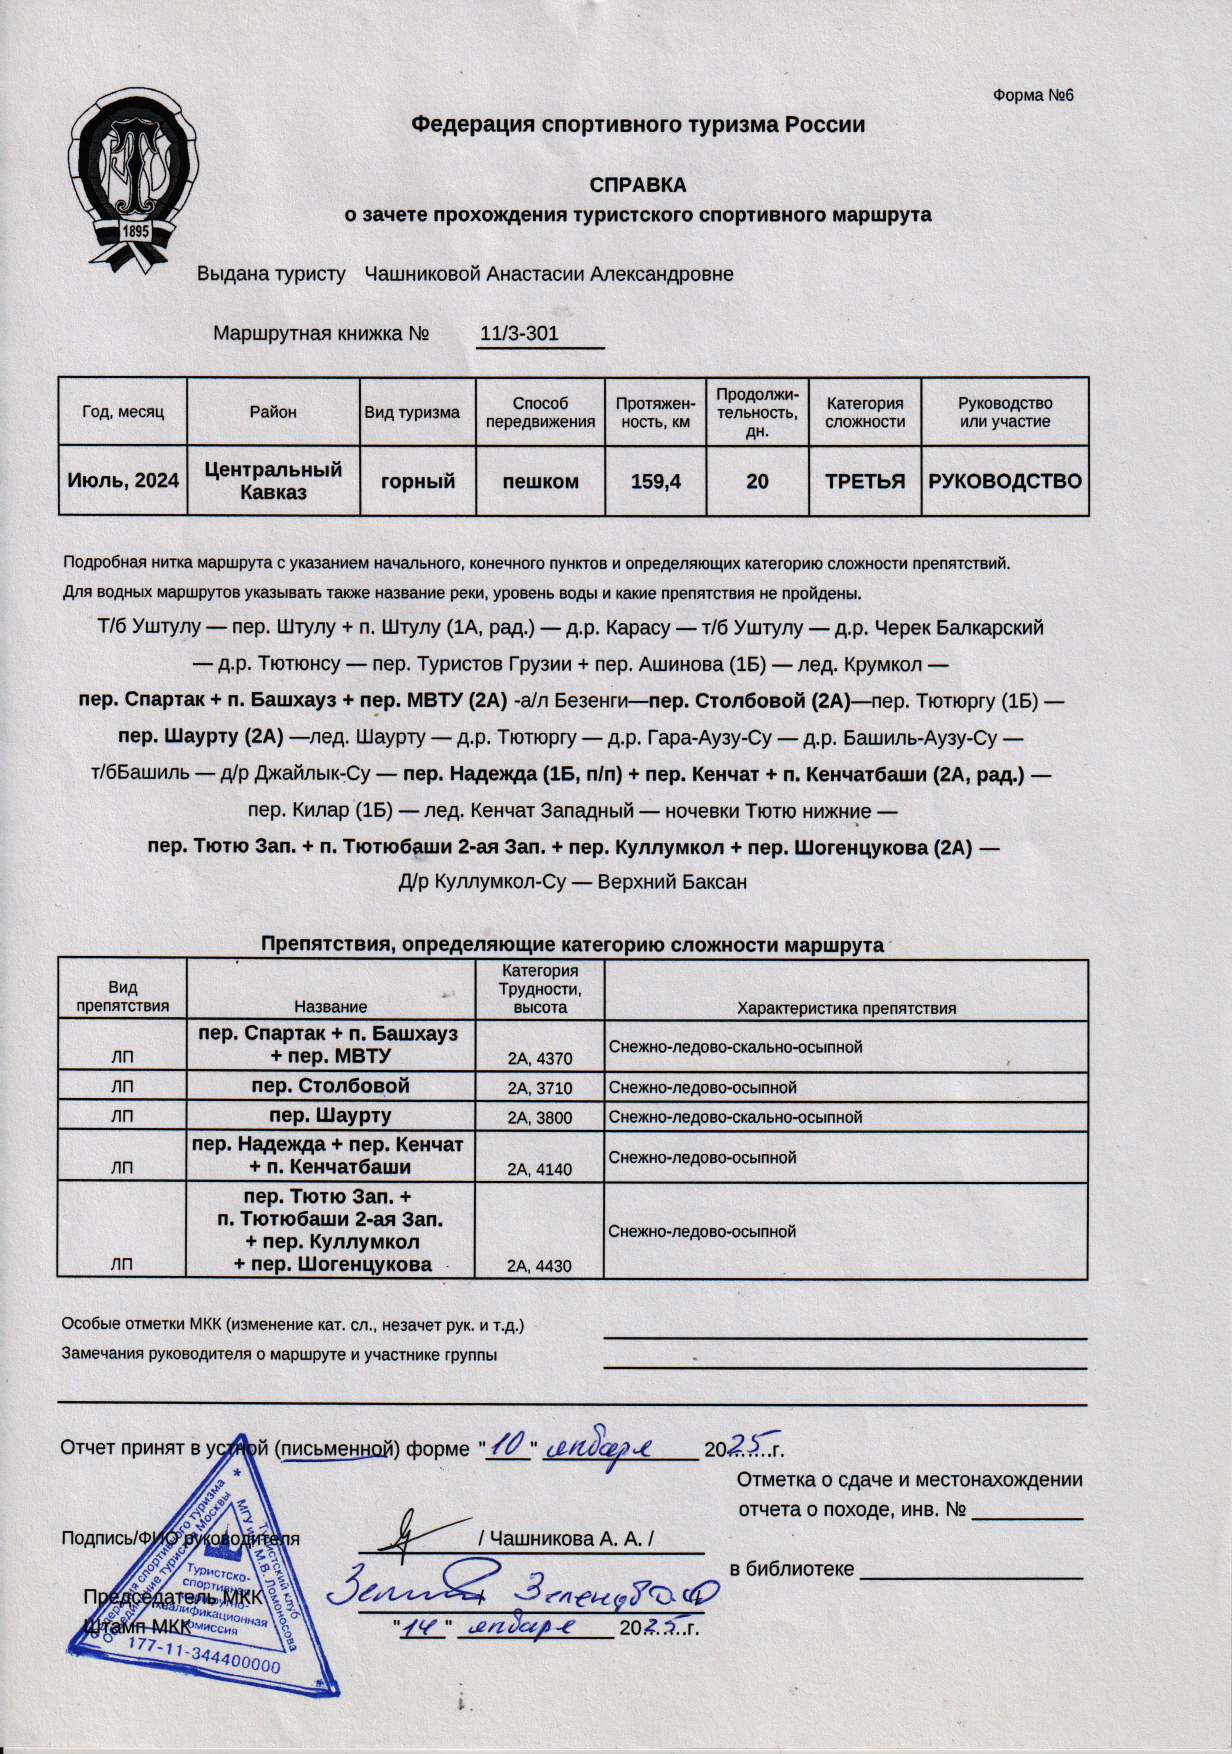
\includegraphics[width=3.5cm]{Pictures/Chapter1/Nastya.png}\raisebox{-1\height}{\rule{0pt}{5pt}}}	&	Чашникова Анастасия Алекссандровна		&	Руководитель				&	1998			&	4ГУ, 2ГР	\\ \hline
			\raisebox{-0.05\height}{\rule{0pt}{155pt}\includegraphics[width=3.5cm]{Pictures/Chapter1/Dima.png  }\raisebox{-1\height}{\rule{0pt}{5pt}}}	&	Коротков Дмитрий Юрьевич				&	Реммастер					&	2001			&	3ГУ, 1ГР	\\ \hline
			\raisebox{-0.05\height}{\rule{0pt}{155pt}\includegraphics[width=3.5cm]{Pictures/Chapter1/Dasha.png }\raisebox{-1\height}{\rule{0pt}{5pt}}}	&	Короткова Дарья Алексеевна				&	Завпит						&	2002			&	2ГУ			\\ \hline
			\raisebox{-0.05\height}{\rule{0pt}{155pt}\includegraphics[width=3.5cm]{Pictures/Chapter1/Katya.png }\raisebox{-1\height}{\rule{0pt}{5pt}}}	&	Мерчи-Байрамова Екатерина Вячеславовна	&	Логист						&	2002			&	2ГУ			\\ \hline
			\raisebox{-0.05\height}{\rule{0pt}{155pt}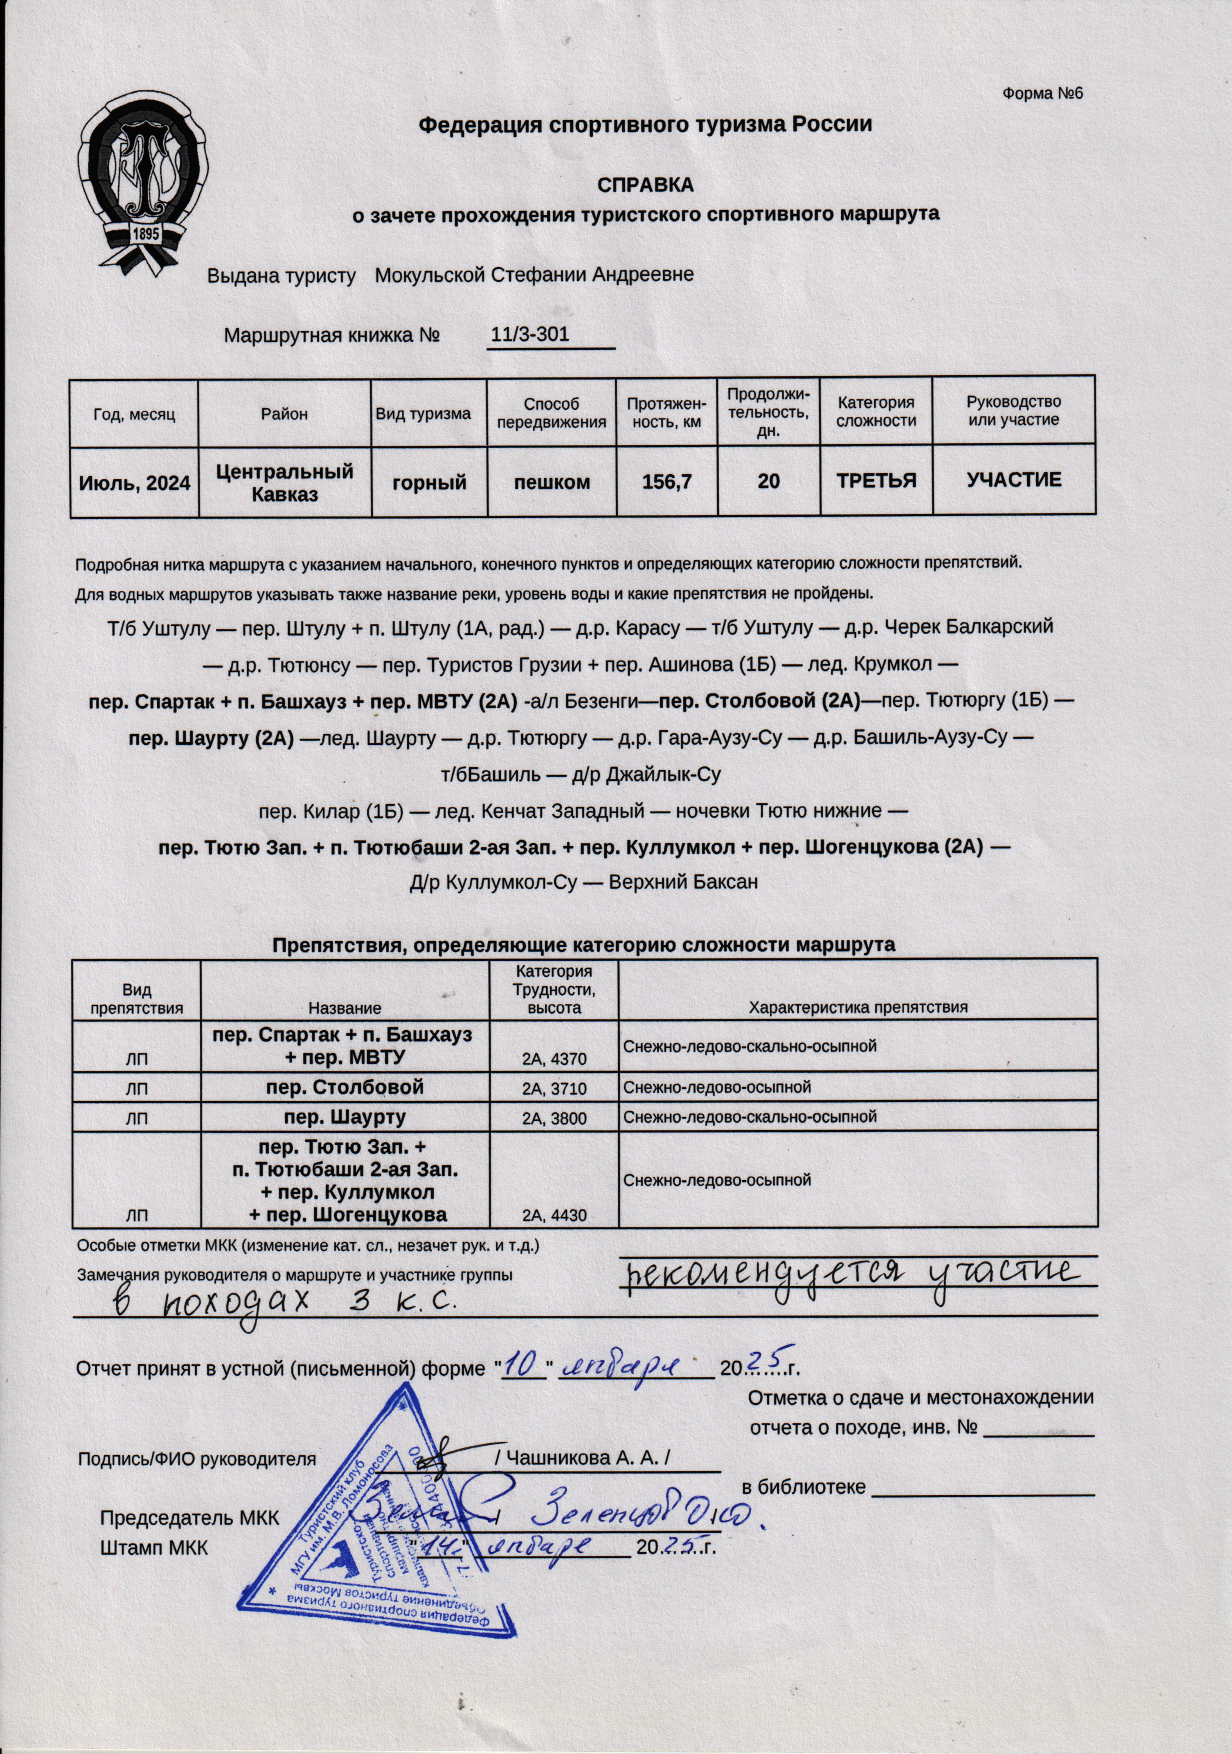
\includegraphics[width=3.5cm]{Pictures/Chapter1/Stepha.png}\raisebox{-1\height}{\rule{0pt}{5pt}}}	&	Мокульская Стефания Андреевна			&	Медик, фотограф				&	1997			&	2ГУ			\\ \hline
			\raisebox{-0.05\height}{\rule{0pt}{155pt}\includegraphics[width=3.5cm]{Pictures/Chapter1/Lesha.png }\raisebox{-1\height}{\rule{0pt}{5pt}}} 	&	Ткачёв Алексей Владимирович				&	Штурман						&	1988			&	2ГУ			\\ \hline
			\raisebox{-0.05\height}{\rule{0pt}{155pt}\includegraphics[width=3.5cm]{Pictures/Chapter1/Yura.png  }\raisebox{-1\height}{\rule{0pt}{5pt}}}	&	Цимбалов Юрий Александрович				&	Снаряженец, хронометрист	&	1989			&	4ГУ			\\ \hline
		\end{longtable}\fxnote{Найти нормальные фотки}

		Поход пройден группой в полном составе. Коротков Дмитрий и Короткова Дарья не участвовали в радиальном выходе на
		вер.~Штулу-Тау (дошли до высоты 3400\,м). Коротков Дмитрий, Короткова Дарья, Мокульская Стефания не участвовали
		в радиальном выходе на пер.~Надежда + пер.~Кенчат + вер.~Кенчатбаши.
		
